\chapter{NLG Tasks}\label{chap:tasks}
Transforming non-linguistic data into grammatically correct sentences in a given language seems like a rather complicated problem. Therefore it is convenient to divide the initial problem into smaller tasks, which are easier to solve. This task structure is described by \citet{reiter1997building} and it is widely used to cover every challenge a fundamental NLG system should deal with:
\begin{itemize}
	\item Content determination 
	= deciding what information will be conveyed
	\item Discourse planning = determining the order of the information
	\item Sentence aggregation = grouping information into sentences
	\item Lexicalization = determining how to express the information in a given language
	\item Referring expression generation = choosing words to express entities
	\item Linguistic realisation = transforming constituents in order to form a well-built sentence in a given language.
\end{itemize}

In this section we will discuss every task mentioned above. The reason we describe every task individually is to highlight challenges that will arise along the way of creating the NLG system. Understanding these tasks is a crucial aspect to produce a well-built software regardless of the choice of the approach (closely discussed in \autoref{chap:approaches}). To illustrate the problems we show numerous simple examples that should ease the process of fully recognizing the extent of issues related to each task.

\section{Content determination}
The goal of this task is to decide what information from input data should be included in the text. Usually the range of the input data is significantly larger than the amount of information we would actually transfer to the user. Naturally, this task is heavily influenced by the specifications of the assignment, namely domain, intention of the text and target audience.

The result of the content determination is usually outputted as a set of preverbal messages, carrying semantic meaning of the statement. To carry all the information an implementation that can describe abstract concepts such relations between statements, entities or conditions is needed. This sub-task of creating suitable representation is usually domain-dependent. Since the important semantic information is mapped into some formal language, there is no need for (human) language to be specified, and therefore this task is language-independent. Concrete examples of formal representation language used to store these semantic attributes are for instance logical language, attribute-value matrices or graphs.

Example of the result of possible content determination is shown below in \figref{cd}, where we would like to choose the content to report one simple message: a goal being scored in a football domain. We have two related (3) sets of attribute-value pairs: (1) is about a player and (2) contains goal statistics. Obviously some information in tables (1) and (2) are too specific (e.g. height of the player) for the message to convey and therefore redundant. Bold attribute-value pairs are highlighted as the ones to be present in the final text (ids are bold to stress their importance, however, we do not output them), creating preverbal message (4) in pseudocode. After performing the remaining NLG tasks possible result could look like (5). 

\begin{figure}[h]
	\centerline{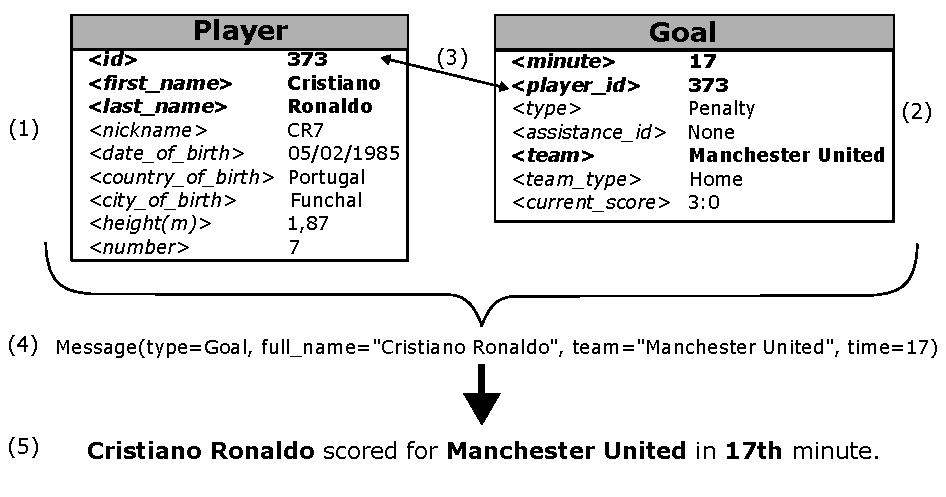
\includegraphics[width=0.95\textwidth]{./img/content_determination.pdf}}
	\caption{Process of content determination}
	\label{fig:cd}
\end{figure}

\section{Discourse planning}
Previous part determines what messages will be transmitted to the reader and this part resolves the issue of the order in which the information is presented. This process is also referred to as text or document structuring. Selecting the right sequence of messages is crucial for text to accomplish its goal. Similarly we structure academic texts to logically ordered paragraphs, which present the topic in a way as understandable as possible for the reader to gain knowledge.

As in content determination, this task is highly domain-dependent as we have to know how to order messages. For instance, a medical report (as an example mentioned earlier) would likely display diagnoses and order decreasingly by how dangerous and life threatening they are. On the other hand, a report from a business meeting could start with a brief overview of achievements and goals and then with issues that were discussed ordered chronologically to allow the reader to follow the course of the meeting.

Human brain orders information to be conveyed in a speech intuitively, but the process as an algorithm itself is not quite trivial. Most common method is to create rules based on the specific domain since the suitable structure heavily relies on the domain. Some researchers suggest using machine learning techniques for creating a  uniform algorithm independent of the domain as seen in \citet{dimitromanolaki2003learning}.

Form of the output of discourse planning can differ. One possible option as described by \citet{reiter1997building} is a tree structure. Leaves of the trees are messages and inner nodes describe specifics of their function in a sentence. This may seem like an unnecessary complicated solution when clustering messages to be said in one sentence can be just an array of messages. The benefit of the tree structure is the amount of information we can store along the messages including constraints under which the message can be said, relations between them and their overall structure.

\section{Sentence Aggregation}\label{section:sa}
The cardinality of the relation message and sentence is rarely one-to-one. Usually multiple messages are formed into one sentence. This process is called sentence aggregation and it is fundamental for generating text that is readable and flows well. To clarify we provide set of verbal messages:
\begin{enumerate}
	\item \emph{Arsenal beat Chelsea.}\label{sa-one}
	\item \emph{Arsenal beat Leeds.}\label{sa-two}
	\item \emph{Arsenal lost to Everton.}\label{sa-three}	
\end{enumerate}

This set of sentences is clearly non-optimal and can be aggregated in two steps as follows:\footnote{\label{footnote-opt}Naturally, no such concept as ``optimal" sentence exists. The optimum in this case is to express the information in a sentence that would likely occur in a spoken human language and also would appear fluid and natural.}
\begin{enumerate}[resume]
	\item \emph{Arsenal beat Chelsea and Leeds. Arsenal lost to Everton.}\label{sa-four}
	\item \emph{Arsenal beat Chelsea and Leeds, but lost to Everton.}\label{sa-five}	
\end{enumerate}

We can notice two types of aggregation leading to optimal sentence (\ref{sa-five}) from sentences presented. Aggregation of:
\begin{itemize}
	\item \textbf{constituents} -- Constituents that have equal syntactic importance can be aggregated using suitable coordinating conjunctions expressing their relation. Take example sentences (\ref{sa-one}) and (\ref{sa-two}). \emph{Chelsea} and \emph{Leeds} are both teams \emph{Arsenal} beat so their semantic meaning is identical. Therefore they can be aggregated via cumulative conjunction \emph{and} creating a new noun phrase in the result sentence (\ref{sa-four}) \emph{Chelsea and Leeds}. Another example of cumulative conjunctions is \emph{both ... and} or \emph{as well as}.
	\item \textbf{sentences} -- Sentences can be aggregated as well using coordinators as seen in the result sentence, which was created by inserting an adversative conjunction in between sentences in example (\ref{sa-four}) to express opposition. This contrast can be expressed by other words like \emph{but}, \emph{yet}, \emph{while}, etc. More relations can be expressed when aggregating sentences using other kinds of coordinating conjunctions: alternative (\emph{or}, \emph{either ...or}, \emph{nor}) to express two or more alternatives and illative (\emph{for}, \emph{so}) to express interference or consequence.
\end{itemize}

Another type of aggregation can occur based on explicit hand-crafted domain-based rules. Take these three preverbal messages from football domain reporting a goal, which are similar to the one as used in \figref{cd}-(4) (Manchester United shortened to MU):
\begin{enumerate}[resume]
	\item \texttt{(type=Goal, full\_name="Cristiano Ronaldo", team="MU", time=4)}\label{sa-six}	
	\item \texttt{(type=Goal, full\_name="Cristiano Ronaldo", team="MU", time=8)}\label{sa-seven}
	\item \texttt{(type=Goal, full\_name="Cristiano Ronaldo", team="MU", time=14)}\label{sa-eight}	
\end{enumerate}

Surely realising messages (\ref{sa-six}), (\ref{sa-seven}) and (\ref{sa-eight}) as three different sentences would not create fluid and natural results as sentences would vary only in time of the goal. Since three goals in football form a so called hat-trick we could aggregate messages in one sentence:

\begin{enumerate}[resume]
	\item \emph{Cristiano Ronaldo completes hat-trick for MU in under 15 minutes.}
\end{enumerate}

This aggregation realises the messages (\ref{sa-six}, \ref{sa-seven}, \ref{sa-eight}) beautifully as the result is well-formed and natural. Notice that the aggregation happened also in expressing the time of the goals: instead of mentioning three different timestamps the time is summarised as \textit{under 15 minutes} highlighting the fact that this rare figure was achieved in a short amount of time. As described in the previous section, football domain knowledge is necessary to decide what is ``long", ``short" or ``average" (and therefore not worth mentioning) amount of time for an event to happen.

Note that these aggregations are simple for humans, but to perform them in a NLG system we need some semantic knowledge and relations of the sentences (or constituents). The easiest approach is to define domain-specific constraints when to perform aggregation. Defining complex domain-independent rules and universal representation of relations is rather a difficult task and nowadays often solved using data-driven methods, which are described later in \autoref{chap:approaches}. 

Furthermore, the idea that the more aggregations we perform the better the final text is wrong. Sometimes slowing down the flow of information by fracturing the message into smaller individual sentences is useful in order to produce more understandable text. Overloading sentences can often result in less fluency as the more information is conveyed in one sentence the harder it is for a reader to follow. \citet{barzilay2006aggregation} are perceiving this as a linear programming problem where similarity is classified for each pair of database entries. Using this similarity, transitivity and global constraints (e.g., maximum number of aggregation across the document) they find an optimal solution.   

\section{Lexicalization}
After performing discourse planning and sentence aggregation the preverbal messages are in a correct order and they contain suitably aggregated information. Goal of this task is to create mapping from these messages to specific expressions in a given human language. This task is the first that is language-dependent. There are two main problems associated with lexicalization. Firstly, the amount of combinations of how to narrate a message is enormous, only restricted to those that fit into the given context. And secondly, transformation of concept into a word (or more words) is very abstract and interferes with many layers of the language (semantics, phonetics and pragmatics) and therefore choosing a suitable expression is rather difficult. This transformation is not even easy for humans. Imagine an essay contest in grammar school with a given topic of the essay. If the transformation was easy and had only one solution, the contest would not exist as essays would be identical. In fact, the perspective and overall understanding of the topic, style of describing one’s point of view and finally even choosing words to present the idea is partly what distinguishes us as people. 

Another factor is the target audience and the overall goal of the language. If the target audience is educated on the matter then using adequate technical terminology is reasonable. Contrastingly, for low-skilled readers all terminology must be explained in an easy way and the content of the text should be more about overall ideas rather than about specific concepts. 

Trivial approach to this task is to hand-craft pairings of a word or a whole phrase and a concept in a message. This solution results in monotonic outputs as the aspect of choice is missing. Slight improvement would be to add more semantically similar options for each item. However, this can cause problems. First of them is how to decide, which possibility is the best. Second is the possible non-viable combinations of words together. One example, that may be not visible on the first glance, is generation of adjectives interpreting numbers. For example, take a player with height of 185 cm. If it was a man, the height is ``average", while a woman could be described as ``tall". Therefore semantic background and suitable comparison need to be taken into account. What is more, combinations of chosen phrases may result in non-realisable or simply weird expressions. 

Due to the vagueness and coherence of the process, NLG systems combine lexicalization, REG and linguistic realisation under one operation called surface realisation or tactical part of the process.  

\section{Referring expression generation}
Referring expression generation (REG) is a process, when you choose words to express domain entities or other constituents of the message. Naturally, utilising one noun phrase for one specific entity, which is used more than once in a short amount of text, results in less readable and fluid text. On the contrary, there is a limit to how many such expressions we can generate since a reader needs to identify the entity correctly. Ambiguity is a highly unwanted effect since the information that needs to be conveyed may differ from its actual language semantic meaning.

To fully understand the challenges and also possible solutions for REG here is an example of sentence where we would like to lexicalize its subject represented as an entity in pseudocode:
\begin{center}
	\texttt{(entity=Player, name="Cristiano Ronaldo”)} \emph{scored a goal for Manchester.}
\end{center}
This particular player can be lexically expressed in this sentence for example as:
\begin{enumerate}
	\item \emph{Cristiano Ronaldo} \label{reg-1}
	\item \emph{Ronaldo} \label{reg-2}
	\item \emph{CR7} \label{reg-3}
	\item \emph{Player number 7} \label{reg-4}
	\item \emph{Portuguese star} \label{reg-5}
	\item \emph{Lately heavily criticised, yet still elite superstar forward} \label{reg-6}
	\item \emph{He} \label{reg-7}
	\item \emph{This player} \label{reg-8}
	
\end{enumerate}
Notice the linguistic techniques we used to express this subject:
\begin{itemize}
	\item \textbf{Entity name} -- Using the name of the entity is a trivial solution and works fine as seen example (\ref{reg-1}).
	\item \textbf{Synonyms} -- Using a synonym or a different name having the identical semantic meaning for the entity as shown in example (\ref{reg-2}) and (\ref{reg-3}). 
	\item \textbf{Descriptive transcription} -- Using the knowledge about the entity (such as physical appearance, characteristics, origin, current events, etc.) we can describe the entity without any need of using its initial name as shown in examples (\ref{reg-4}), (\ref{reg-5}) and (\ref{reg-6}). Although expression (\ref{reg-4}) identifies Ronaldo unambiguously among Manchester United players, the description  may be too specific for a reader with less knowledge about football. Therefore the target reader, his knowledge about a topic and also the purpose of the text are important even in this task. This technique is also prone to ambiguity as seen in example (\ref{reg-5}): reader should already know what player is being described in the text to use this expression since more players can be characterised as \textit{Portuguese star} among Manchester players (e.g., Bruno Fernandes) .
	\item \textbf{Definite descriptions} -- The expression can be enriched by adding valid adjectives, adverbs or other linguistic structures to further specify the object as seen in example (\ref{reg-6}) where adjectives \textit{criticised} and \textit{elite} add more information about the player. Note that this principle is used even for the adjectives: \textit{criticised} \textrightarrow \textit{Lately heavily criticised}, \textit{elite} \textrightarrow \textit{still elite}. Finally, adding adversative conjunction \textit{yet} creates enriched and complex noun phrase.
	\item \textbf{Pronouns} -- In a human language pronouns are used to represent entities as seen in (\ref{reg-7}), (\ref{reg-8}). Using pronouns correctly can help to improve readability of the text and also minimise the obvious flags of computer-generated text. The main obstacle to overcome is when to use pronouns. Sometimes usage of a pronoun can arise from context, sometimes if there is absolutely certainty that everyone knows what the pronoun is referring to: those examples are hard to deal with and usually handled explicitly. Usual approach is to use pronoun if the entity was mentioned in a previous sentence under the condition the entity was the only constituent the pronoun could refer to.
\end{itemize}

How to approach REG depends also on repetition of the entities in the text and the final text variability. In a domain where identifying the entity unambiguously is primary the usage of REG is even harmful. For instance, expressing city ``New York, USA" as ``The city that never sleeps" in the air travel domain, where the clear identification of city is a necessity. To the contrary, expressing an entity identically multiple times in a short span of prosaic text eventuates in dull, plain and stereotypical language. 

\section{Linguistic realisation}\label{section:lr}
Realisation is responsible for the non-trivial task of expressing each lexical item in the sentence in terms of its morphological, syntactic, and potentially also phonological and phonetic properties. This process requires changing words to a valid form, adding auxiliary words (prepositions, verbs, etc.), handling agreements, ordering, inserting punctuation and other similar transformations all in order to present the language not only factually, but even grammatically correct. Implementation of a realisation system is strongly dependent on the target language as shown below.

Firstly, we present an example to illustrate complexity of this task. Secondly, we state a brief example that languages around the world can behave differently. Then we describe a few approaches to the solution of realisation. 

\subsection{Example: numeral constructions}
Consider the problem of building a noun phrase including a numeral:
\begin{enumerate}
	\item \texttt{(entity=Animal, name ="dog", count=1)} $\rightarrow$ \emph{one dog} \label{lr-1}
	\item \texttt{(entity=Animal, name="dog", count=23)} $\rightarrow$ \emph{23 dogs} \label{lr-2}
	\item \texttt{(entity=Animal, name="mouse", count=2)} $\rightarrow$ \emph{two mice} \label{lr-3}
	\item \texttt{(entity=Animal, name="fish", count=1000)} $\rightarrow$ \emph{thousand fish} \label{lr-4}
\end{enumerate}

Trivial and also naive solution for this simple noun phrase building can be to append morpheme ``\textit{s}" to the name of the animal if the count is more than one. As you can see in example (\ref{lr-3}) and (\ref{lr-4}) this solution can work only for animals that have regular plurals. In addition, the count itself is recommended to be expressed by a word and not by numeral if the number is either a small integer (1-10) (examples \ref{lr-1}, \ref{lr-3}) or a well-known rounded number (hundred, thousand, billion, etc.) shown in (\ref{lr-4}). On the other hand, example (\ref{lr-2}) uses a number. Therefore we need to implement a more complex system that resolves all of these issues.

\subsection{Languages differences}
One, so far omitted, important aspect are the principles of morphology and syntax of the language. Concept of appending morpheme to express plural might not be so easily transferable into different languages. In Slavic languages morphemes to express plural differ and also can be infixed, meaning they could be inserted into the word stem instead of using a suffix. In Czech, a word for dog is \emph{pes}. Then realising their number would look like: \emph{1 pes, 2 psi, 5 psů}. Slavic languages are synthetic, meaning a word usually consists of more morphemes carrying multiple grammatical, syntactic or semantic meanings. Furthermore, an agreement between the grammatical case and the noun is resolved as well with an infix morpheme. Here are three examples in Czech using different grammatical cases along with translation from English to further showcase complexity of the task:

\begin{itemize}
	\item (case: nominative) \emph{two \textbf{dogs}	$\rightarrow$ dva \textbf{psi}}
	\item (case: genitive) 	\emph{without two \textbf{dogs}  $\rightarrow$ bez dvou \textbf{psů}}
	\item (case: instrumental) \emph{with two \textbf{dogs} 	$\rightarrow$ s dvěma \textbf{psy}}
\end{itemize}

Synthetic languages are just one specific type of languages based on the division according their morphological typology. Subtype of such languages are polysynthetic languages (e.g., Inuit languages), where words are constructed by combining a huge number of morphemes representing a complex expression, possibly a whole sentence. In central Nunavut Inuktitut \emph{Tusaatsiarunnanngittualuujunga} means \emph{I cannot hear very well}. Complete opposites are analytic languages (e.g., Vietnamese), where morpheme-to-word ration is nearly one. 

The extent of language influence is huge even in the semantic part as well. To demonstrate, imagine generating a sentence, in which the action will happen in the future. However, English, unlike Romance languages (French, Spanish, Italian and more) does not have future grammatical tense and we have to use other structures to express future (will, be going to, present continuous or simple present). Some languages are even tenseless, e.g. Tokelauan spoken in American Samoa (Polynesia).

Languages can be divided into groups based on numerous criteria. This section only cherry-picked a few aspects we can observe and their listing is definitely not exhaustive. Purpose was to give an idea about the diversity of languages around the world. Also we illustrated the need for the analysis of language principles during the linguistic realisation to be able to propose a fully-functioning solution.  

\subsection{Templates}
First approach to the realisation problem is exploiting templates. Templates are typically hand-crafted using fixed lexical items and attributes substituted in the template. Preverbal message (\ref{lr-t-1}) is assigned to a template (\ref{lr-t-2}) and three variables are then substituted with values creating the target sentence (\ref{lr-t-3}). 

\begin{enumerate}[resume]
	\item preverbal message -- Message(type=Goal, full\_name = "Cristiano Ronaldo", team = "Manchester United", time = 17) \label{lr-t-1}
	\item template -- \textbf{\$full\_name} \emph{scored for} \textbf{\$team} \emph{in} \textbf{\$minute}\emph{th} \emph{minute}. \label{lr-t-2}
	\item result -- \textbf{Cristiano Ronaldo} \emph{scored for} \textbf{Manchester United} \emph{in} \textbf{17}\emph{th} \emph{minute}. \label{lr-t-3}
\end{enumerate}

The advantage of this approach is simplicity and prevention of grammatical errors considering that we have full control of what the fixed segments are and any unwanted error is highly improbable. The disadvantages prevail. First of all, applying templates could be only feasible in well-defined low-volume domains as entities must have easy-to-text-interpretation. Another reason is that creating templates is time-consuming. And most importantly, the variation of the output is low as the immutable parts of the text generate very limited output. In addition, the template approach for more complicated languages tends to struggle, because the constituents usually depend on each other (e.g. agreement, auxiliary words, etc.) creating requirements, whose combinations are hard to fulfil. 

However, templates are extremely practical when the target output is expected to be simple and 
rarely changing. Great example is generating spoken announcements in the transportation domain e.g., departures of flights on the airport, where the template could look like: \emph{The departure of flight number} \texttt{\$number} \textit{from} \texttt{\$destination\_from} \textit{to} \texttt{\$destination\_to} \textit{will be slightly delayed.} $\rightarrow$ \textit{The departure of flight number \textbf{FD-2018} from \textbf{Rome} to \textbf{Paris} will be slightly delayed}. Results are admittedly blunt in terms of language richness, but they are factually correct, clear and easy to comprehend, which was the initial purpose.
    
\subsection{Other approaches}
Other approaches are more complicated in order to outperform templates in a range of expressions.  First of them is building a grammar for the natural language. This approach relies on thorough knowledge and examination of the language behaviour and principles offering domain-independent solutions that can be applied to a different NLG system performing linguistic realisation. The advantage of this approach is definitely the domain independence of the realiser as well as its variety in produced output. Disadvantage is that building such grammar is labour-expensive and the disability to select the best possible result. All generated sentences will be correct, but the choice, which one is the optimal one is beyond grammar's reach.

Secondly, data-driven (further described \autoref{chap:approaches})methods can be applied in this task too. However their usage can vary greatly. Both approaches above can be enhanced by these stochastic methods since we can reduce manual workload. Templates can be automatically extracted from training corpus (more about corpora in \autoref{chap:process}). Similarly, hand-crafted grammars can be created automatically from corpora. Also, linguistic approaches can be avoided by using these methods. However, fusing traditional linguistic approaches and the power of statistical approach can result in a well-performing system. For instance, using hand-crafted grammar in combination with stochastic methods to resolve the optimal-among-the-correct-ones issue.


